% Latex Style for CMP PGR DAY 2009.
%
% Revision 1.0
% Feb. 12 2009.
%
% Barry-John Theobald, University of East Anglia, Norwich, UK

\documentclass{cmppgr}

\usepackage[pdftex]{graphicx}
\graphicspath{{figures/}}

\input{t1pcr.fd}
\makeatother
\setlength{\footnotesep}{3ex}
\usepackage{listings}
\usepackage{pgfplots}


\title{Probabilistic approach over Decision Trees for problems with discrete data with a small number of instances 2017 --- Norwich, UK}
\name{Luke M. Garrigan}
\institution{
	Machine Learning, University of East Anglia, UK
}
\email{l.garrigan@uea.ac.uk}



\begin{document}
\maketitle

\begin{abstract}

Bayesian classifiers are widely known for their optimality when attributes are independent given the class. This paper attempts to prove that small samples of discrete data with arbitrary dependencies are more accurately classified using a probabilistic approach over decision trees. 


\end{abstract}

\keywords{Probabilistic, Naive Bayes, Decision Trees}

\section{Introduction}

In machine learning a learner algorithm is given a set of training instances with their corresponding class labels, it then produces a classifier. The classifier takes unlabelled testing instances and assigns it to a class. Choosing the best suited algorithm specific to the sample set is not a trivial process. 

Probabilistic classification is the application of approximating a joint distribution with a product distribution. Bayes rule is used to approximate the conditional probability of a given class label. Approaches such as \textit{naive} Bayes are among the most popular classifiers used in the machine learning community, derived from generative probability models they are generally easy to understand and the induction of these classifiers is extremely fast, requiring only a single pass through the data if all attributes are discrete \cite{kohavi1996scaling}. The \textit{naive} Bayes classifier is the simplest of models in this paper, it assumes that all attributes are independent of each other given the context of the class. Although the \textit{naive} assumption of independence is not true in terms of most sample sets, many papers such as \cite{domingos1997optimality} have proven that \textit{naive} Bayes classification accuracy is very competitive when compared with more complex state-of-the-art algorithms. 
$$ P(A \mid B) = \frac{P(B \mid A) \, P(A)}{P(B)} $$
 

Decision trees classify instances by sorting them down the tree from the root to some leaf node which represents the classification of the given instance. Nodes specify a test of some attribute of the instance and each branch from that node corresponds to one of the possible values for this attribute. A given instance is classified moving down the tree, the attribute specific to that node is tested. Following down the branch corresponding to the value of the attribute in the given example, this is then repeated until a leaf node is reached and a classification is made.

 


\section{Data Description}

\subsection{Discretization}
Discretization concerns with the process of transferring continuous data into discrete counterparts. Numeric attributes were discretized into ten equal-length intervals, unless the number of uniquely observed values for an attribute was less than 10. This approach was compared in \cite{dougherty1995supervised} with entropy-based and purity-based methods, which are supervised algorithms. An empirical evaluation showed that the \textit{naive} Bayes algorithm significantly improved accuracy when features were discretized using an entropy-based method. However due to its simplicity the unsupervised binning discretization method was used.

\subsection{Methods For Accuracy Estimation}







\subsubsection{K-Fold Cross-Validation}
Cross-validation is a computationally expensive algorithm used to estimate performance, it uses all available instances as both training and testing sets. The dataset is split into $k$ equally sized non-overlapping subsets $S$. Given a fold $S_i$ a model is trained on $S \setminus S_i$, then $S_i$ is used to create the accuracy estimation.

\subsubsection{Leave-One-Out Cross-Validation (LOOCV)}
Leave-One-Out Cross-Validation is  K-fold cross validation where $K$ is equal to the number of instances in the dataset. The classifier is trained on all data expect the one instance being left out and the prediction is made. An average of the data is collected and used to evaluate the classifier. 

\subsubsection{Bias And Variance Tradeoff}
As $k$ increases the less bias the classification is in overestimating the true expected error because the folds will be closer to the total dataset. However in doing this it induces a significant amount of variance. To minimise the testing bias a large portion of the dataset must be used for training, meaning not much data is used for testing, this ensures that the model will be as close as possible to the the one that would be achieved from training using the entire dataset. Minimising the testing variance would mean quite the opposite, so a large amount of data would be used for testing, this ensures a more reliable estimate of error of the classifier.

 

Due to the small sample sizes 10-fold cross-validation was used as an estimator in an attempt to minimise the estimation variance.


\begin{table}[h]
	\centering
	\caption{An example table.}
	\begin{tabular}{|l|c|c|}
		\hline
		Data Set & Instances & Attributes \\\hline\hline
		Echo cardiogram & 131 & 13\\
		Teaching Assistant & 150 & 6\\
		Seeds & 209 & 8\\
		Planning Relax & 180 & 13\\
	    Hepatitis & 154 & 20\\
		Breast Cancer & 284 & 10\\
		Ecoli & 223 &10 \\
		Glass & 141 &6  \\
		Haberman & 203  &4 \\
		Hayes Roth & 158 &5 \\
		Heart & 169 & 14\\
		Lymphography & 156 &19 \\
		Promoters & 104 &58  \\
		Shuttle Landing & 252  &7 \\
		Sonar & 137 &61 \\
		Thyroid & 142 & 6\\\hline
	\end{tabular}
	\label{tab:example}
\end{table}




\subsection{Sections}

Section headings should be centred on the line, be in bold typeface, and only the first letter should be capitalised. Sub-headings are also in bold face, but appear flush left and are typeset in the base font size. Sub-sub-headings appear like sub-headings, except they are in italics and are not boldface. No more than 3 levels of headings are allowed.

\subsection{Headers and Footers}

All headers and footers must be left empty. Your document should not contain page numbers etc. These will be added later.

\subsection{Lists}

Itemised lists can be included in your document, but please check the indentation if you are not using \LaTeX. An example itemized list with the correct formatting should look like the following:
%
\begin{itemize}
\item{First list item.}
\item{Second list item.}
\item{Third list item.}
\end{itemize}
%

\subsubsection{List Depth}

Please try not to use hierarchical lists, these look cluttered in two-column format. Keep lists to a single level of depth.

\subsection{Figures}

All figures must be centred on the column (or page, if the figure spans both columns). A figure caption should follow the figure and be formatted like the example in Figure~\ref{fig:columnfigure}.

\begin{figure}[h]
\centering
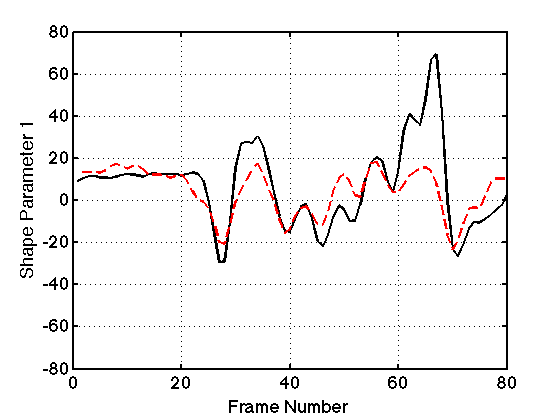
\includegraphics[scale=0.4]{sparam_1_errors}
\caption{An example of a figure centred on a single column. The figure is not centred automatically. To centre the figure, use \texttt{$\backslash$centering} within the \texttt{figure} environment.}
\label{fig:columnfigure}
\end{figure}

Figures spanning multiple columns should appear either at the top or the bottom of the page. You can use the $\backslash$figure* command to span a figure across both columns. An example is shown in Figure~\ref{fig:pagefigure}.

\begin{figure*}[tb]
\centering
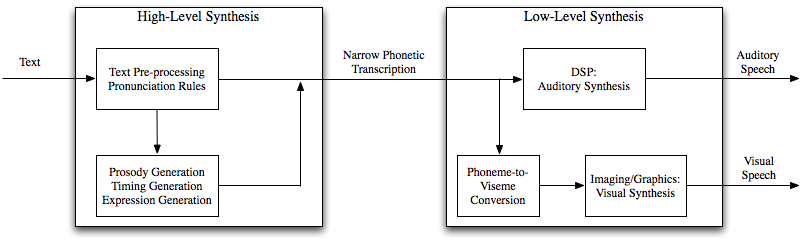
\includegraphics[scale=0.5]{AVTTS-Overview}
\caption{An example of a figure spanning both columns and centred on a page. Again, the figure is not centred automatically.}
\label{fig:pagefigure}
\end{figure*}

Figures should preferably be line drawings. The proceedings will not be produced in colour, so please do not rely on colour to distinguish between curves on a graphs, etc. You should check to ensure the figures print well on a good quality printer, and that there are no issues when colour figures are printed in grey-scale.

Before including any figures in your document you should ensure you have the necessary copyright permission.

\subsection{Tables}

Tables should be centred on a column if possible. There is no strict requirement on the style as this will largely depend on the content to be displayed. An example table is shown in Table~\ref{tab:example}, but this is provided for illustrative purposes only.

\begin{table}[h]
\centering
\caption{An example table.}
\begin{tabular}{|c|c|}
\hline
Trial & Score \\\hline\hline
1 & 10 \\
2 & 12 \\
3 & 11 \\
4 & 9 \\
5 & 11 \\
6 & 10 \\\hline
\end{tabular}
\label{tab:example}
\end{table}

Note, for tables the caption should be above the table, as shown in Table~\ref{tab:example}.

\subsection{Equations}

Equations should appear on a separate line, they should be centred and they should be numbered. Some examples are:
%
\begin{equation}
y = mx + c,
\label{eqn:line}
\end{equation}
%
which obviously is the equation of a straight-line of gradient $m$ and intersecting the vertical axis at $c$. Another famous equation with $m$ and $c$ is
%
\begin{equation}
E = mc^2.
\label{eqn:einstein}
\end{equation}

\subsection{Fonts}

You should use 9 point Times or Times Roman for the main text. All fonts should be embedded in the final PDF document.

\subsection{Hyperlinks}

Hyperlinks should be written in full, e.g., \texttt{http://www.cmp.uea.ac.uk}, and must be coloured black. For ease of readability, authors are advised to use a different font family from the main text.

\subsection{Supplementary Material}

Authors may submit supplementary material with their paper. However, this should not be included in place of a technical description of your work. Reviewers are not obliged to watch video sequences, and your submission will be reviewed on the strength of the paper only. If you are submitting a multimedia file, please use widely accepted formats/codecs. The conference proceedings will not include media players.

\section{Conclusions}

The page limit is 4--6 pages. Please, please use \LaTeX\ to typeset your document. This will minimise any formatting headaches!

\subsection{References}

You must reference any papers you have had accepted or are under review here. Example references~\cite{massaro98:perceiving}, audio-visual speech synthesis~\cite{theobald04:specomm,theobald08:lips}, and audio-visual speech recognition~\cite{cox08:avsp,matthews2002:extraction}.

See the references section for the formatting of the references from different sources (conferences, journals, and books). The formatting of references follows the standard IEEE format, \LaTeX\ users should download the \texttt{IEEEtran} bibliography format. References should be listed in order of citation.

\bibliographystyle{IEEEtran}
\bibliography{sample_bib.bib}

\end{document}
